\documentclass[12pt]{article}
\usepackage{graphics}
\renewcommand{\deg}{\mathrm{deg}}
\newcommand{\kg}{\mathrm{kg}}
\newcommand{\m}{\mathrm{m}}
\newcommand{\s}{\mathrm{s}}
\newcommand{\mps}{\m\,\s^{-1}}
\newcounter{problem}
\begin{document}\sloppy\sloppypar\raggedbottom\frenchspacing\thispagestyle{empty}

\section*{NYU Physics 1---rolling}

A heavy round pipe of mass $m$, radius $R$, and moment of inertia $I$
sits at rest on the horizontal bed of a parked truck, a distance $L$
from the end of the truck bed.  At time $t=0$, the truck starts to
accelerate forwards with acceleration $a$, at which point the pipe
begins to roll without slipping on the truck bed.  Give all your
answers with respect to the stationary ground, {\em not} the moving
truck.
%\\ \rule{0.3\textwidth}{0pt}
%\resizebox{0.4\textwidth}{!}{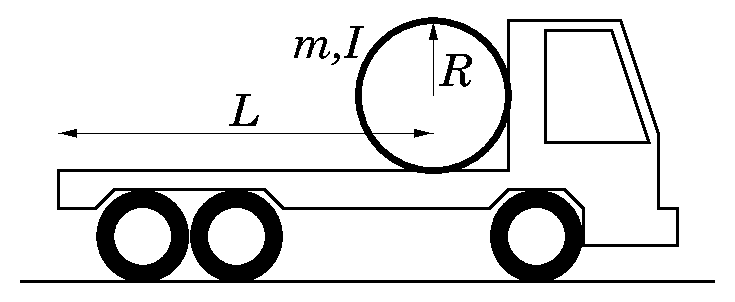
\includegraphics{../eps/truckpipe.eps}}

\textsl{(a)} During the acceleration, when the truck is moving at
speed $v_t$ and the pipe is moving at speed $v_p$ (with respect to the
ground) and the pipe is spinning at angular speed $\omega_p$, what is
the condition (that is, the equation relating $v_t$, $v_p$, $\omega_p$
and $R$) for rolling without slipping on the truck bed?  \emph{Think
about the movement of the pipe relative to the truck bed.}

\textsl{(b)} Draw a free body diagram for the pipe, showing all
forces, for $t>0$.

\textsl{(c)} Which way does the pipe accelerate (relative to the
ground)?  Will its acceleration be greater or less than $a$?  Which
way does it start to spin?  That is, anticipate the dynamics.

\textsl{(d)} What is the acceleration of the pipe?  That is, solve the
equations you have.

\textsl{(e)} When (at what time) does the pipe fall off the truck?

\end{document}
